\section{Background and Challenges}
\label{sec:background}
\subsection{Parameter-Efficient Finetuning}
\label{subsec:peft}
Finetuning enables LLMs to adapt to specific domains and downstream tasks~\cite{devlin2018bert,radford2019language,brown2020language}. However, full finetuning introduces significant computational and memory overheads. To address this, {\em parameter-efficient finetuning} (\peft) methods~\cite{ding2023parameter} have been proposed. 
%
These include prompt embeddings~\cite{liu2023gpt,li2021prefix,lester2021power}, adapter modules, low-rank decomposition (LoRA)~\cite{hu2021lora}, and (IA)$^3$ \cite{liu2022few} scaling of the pre-trained weights. Recent unified approaches also combine various \peft methods using heuristics \cite{he2021towards} or neural architecture search \cite{zhou2023autopeft,zoph2016neural,mao2021unipelt}. While \peft approaches minimize trainable parameters, reducing parameter count is sometimes not enough to reduce the memory footprint.


\begin{figure*}
    \centering
    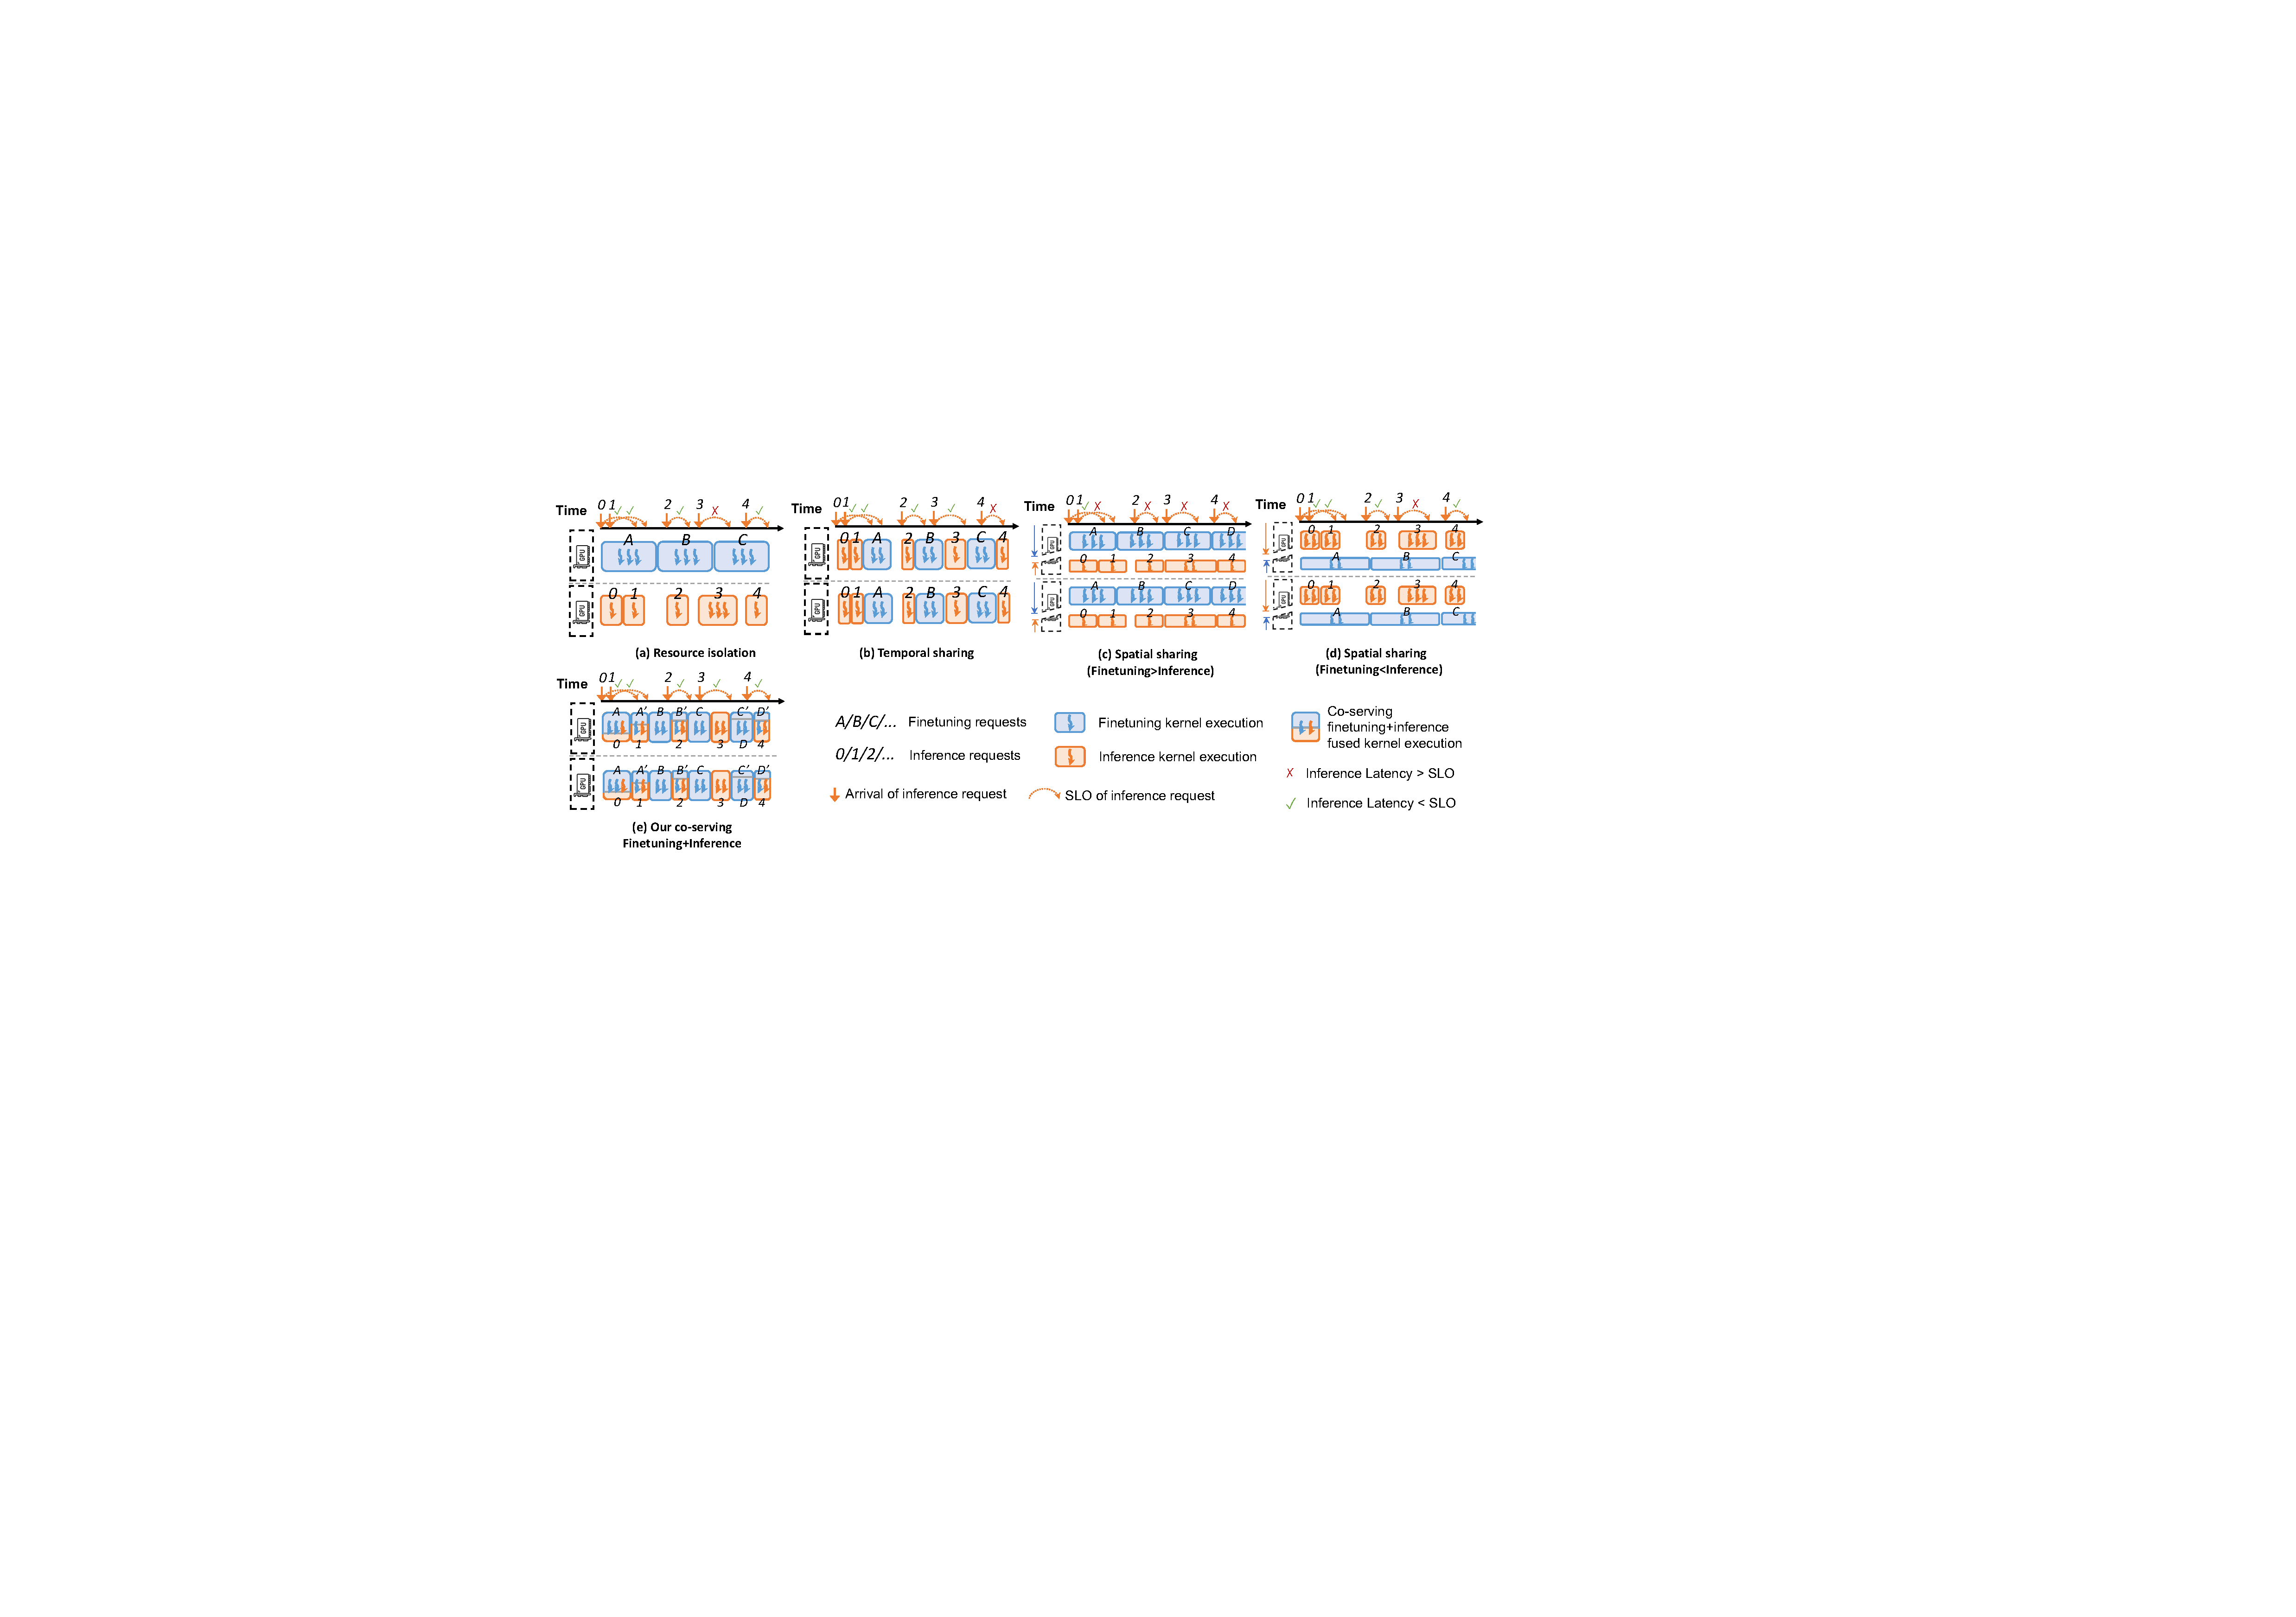
\includegraphics[width=\textwidth]{figs/baseline7.pdf}
    \caption{Comparing different resource sharing approaches for serving finetuning and inference. For spatial sharing and co-serving, the height of rounded rectangles illustrates the splitting ratio of GPU resources (e.g., streaming multi-processors).}
    \label{fig:baseline}
\end{figure*}


\subsection{\peft-based LLM Inference}
\label{subsec:llm_serving}

LLM inference is increasingly essential in research and industrial applications. Recent systems serve multiple \peft-based LLMs simultaneously. For example,PetS~\cite{zhou2022pets} decouples linear layers into shared and task-specific operations, optimizing scheduling for improved throughput.
% 
More recent works focus on optimizations that are specific to generative decoding models. Punica~\cite{chen2023punica} introduces specialized CUDA kernels for multi-tenant LoRA serving. S-LoRA~\cite{sheng2023s} proposes unified paging and heterogeneous batching for thousands of LoRA components. dLoRA~\cite{wu2024dlora} improves efficiency through dynamic batching adjustments.

\subsection{Challenges in Co-serving Inference and Finetuning}
\label{subsec:challenges}
Co-serving inference and finetuning tasks within a single system, as envisioned by \sys, presents significant challenges due to their differing workload characteristics. \Sys must address three key challenges.

First, \emph{how can inference and finetuning tasks be co-located while minimizing the memory footprint}?  
Traditional multi-tenancy ML scheduling systems share resources across tasks and models~\cite{xiao2018gandiva}, but suffer from the high memory demands associated with LLMs.
Furthermore, existing finetuning systems usually retain all intermediate activations similar to training systems to enable gradient computation during backpropagation, which substantially increases their resource consumption compared to pure inference tasks. This discrepancy makes it challenging to manage system resources between finetuning and inference tasks.

\Sys addresses this by co-locating finetuning and inference tasks to share backbone LLM parameters and activation buffers, using {\em dependent parallelization} to optimize the placement of trainable {\em bypass networks} (e.g., LoRA adapters~\cite{hu2021lora}) in a distributed fashion (see $\S$~\ref{subsec:parallelization}) and {\em graph pruning} to eliminate unnecessary data dependencies for frozen parameters (see $\S$~\ref{subsec:pruning}). These optimizations reduce finetuning memory overhead by up to 8$\times$.

Next, \emph{how can we run inference and finetuning tasks simultaneously while minimizing the interference with inference latency and SLO attainment}? 
Previous work on traditional ML workloads~\cite{romero2021infaas} has shown that co-locating inference with training can significantly degrade inference performance.
Unlike conventional training workloads that require coarse-grained temporal or spatial resource sharing~\cite{choi2022serving}, LLM finetuning provides a unique opportunity to batch base LLM computation and parameter access across requests from different finetuned variants~\cite{wu2024dlora}. However, due to differences in execution logic---auto-regressive decoding in inference versus backpropagation in finetuning---merging the two types of tasks remains difficult.
%
To overcome this challenge, \Sys introduces {\em token-level finetuning}, decomposing finetuning sequences into smaller units ($\S$\ref{subsec:incremental_finetuning}) that, during the forward pass, follow the same execution order as inference tokens. In this way, both inference and finetuning tokens can be processed together using fused GPU kernels. For the backward pass, \sys launches separate GPU streams for finetuning tokens and adopts a layer-wise execution strategy to minimize memory usage.

Finally, \emph{how can we handle fluctuating inference workloads while preserving their latency SLO}?
%
Given the dynamic nature of inference request arrival patterns, provisioning for peak demand often results in significant resource under-utilization.
\Sys's fine-grained, token-level execution strategy enables quick adaptation to load fluctuations.
To achieve this, \sys introduces a {\em hybrid token scheduler} (Section~\ref{subsec:scheduler}) that prioritizes inference tokens for SLO compliance while opportunistically inserting finetuning tokens in a best-effort manner to maximize GPU utilization.